\chapter{Análisis y comparativa de paquetes}
\label{cha:analisis y comparativa de paquetes}

Tras la exposición de las diferentes variables y métricas que conformaran la evaluación, se realiza el
correspondiente análisis y comparación de paquetes. Inicialmente, el análisis será individual de cada 
paquete, para finalmente hacer una comparativa conjunta.

\section{Evaluación individual de paquetes}
\label{sec:evaluacion individual de paquetes}

A continuación se realiza un análisis individual de los resultados obtenidos de cada paquete. Adicionalmente, 
se incluyen resultados de otros paquetes con el objetivo de efectuar una pequeña comparación entre los 
mismos.

\section*{inscriptis}

El primer paquete sometido a análisis será \textbf{inscriptis}, el cual debemos instalar e importar en el
fragmento de código respectivo. En cuanto a su instalación, es muy sencilla, simplemente se debe ejecutar
la siguiente instrucción en la línea de comandos: \emph{\$ pip install inscriptis}.

\begin{codefloat}
    \inputencoding{latin1}
    \lstinputlisting[style=CppExample, showstringspaces=false]{scripts/script-inscriptis.py}
    \inputencoding{utf8}
    \caption{Función de ejecución de inscriptis}
    \label{cod:funcion de ejecucion de inscriptis}
\end{codefloat}

En cuanto al código mostrado en \ref{cod:funcion de ejecucion de inscriptis}, es muy simple. Se itera sobre 
los archivos HTML a analizar, y se emplea la función \emph{get\_text()} para obtener la información deseada. 
Dicha información se almacena posteriormente de forma ordenada sobre un diccionario.

Para conservar la información obtenida y no ejecutar el algoritmo múltiples veces, el diccionario obtenido
se almacena en un archivo \emph{json} propio del paquete. De esta forma, el archivo \emph{inscriptis.json} 
conserva todos los fragmentos de texto obtenidos del minado web anterior.

Una vez ejecutado el algoritmo, se realizan todos los cálculos pertinentes y se determinan las puntuaciones
obtenidas. En el caso de \textbf{inscriptis}, se muestran en la tabla
\ref{tab:tabla - resultados de la evaluacion de inscriptis} los resultados obtenidos.

\begin{table}[h]
    \begin{center}
      \begin{tabular}{| c | c | c | c | c | c | c | c |} \hline 
       \textbf{Nombre} & \textbf{Accuracy} & \textbf{Precision}  & \textbf{Recall} & \textbf{F1} & \textbf{RAM(\%)} & \textbf{CPU(\%)} & \textbf{Time Exec.(s)} \\ \hline
       inscriptis & 0.5414 & 0.5404 & 0.9875 & 0.6985 & 45.0 & 0.2 & 2.1005 \\ \hline
      \end{tabular}
      \caption{Tabla - Resultados de la evaluación de inscriptis}
      \label{tab:tabla - resultados de la evaluacion de inscriptis}
    \end{center}
\end{table} 

En forma de gráfica, se muestra en la figura \ref{img:grafica - resultados de la evaluacion de inscriptis}
los cálculos obtenidos en referencia a las métricas independientes del entorno de ejecución. Analizando
estas métricas, y sabiendo que \emph{f1} determina la calidad en general de la extracción, podemos concluir
que \textbf{inscriptis} realiza un equilibrado trabajo en el minado web.

\begin{figure}[tphb]
    \centering
    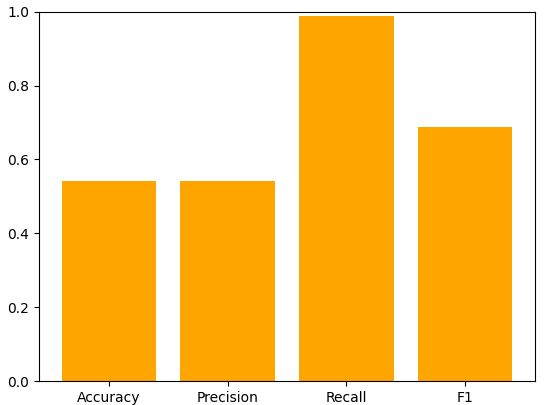
\includegraphics[width=5in]{resultados-inscriptis.jpg}
    \caption{Gráfica - Resultados de la evaluación de inscriptis}
    \label{img:grafica - resultados de la evaluacion de inscriptis}
\end{figure}

Por otro lado, respecto a las métricas dependientes del entorno, al solo tener una medición de referencia 
no podemos decir demasiado. El uso de memoria RAM parece elevado dadas las especificaciones del entorno. 
Por el contrario, el uso de CPU es mínimo. Algo sorprendente es que \textbf{inscriptis} haya sido capaz de 
analizar 101 documentos HTML en únicamente dos segundos.

\section*{Beautiful Soup}

El segundo paquete sometido a análisis será \textbf{Beautiful Soup}, el cual debemos instalar e importar 
en el fragmento de código respectivo. En cuanto a su instalación, es muy sencilla, simplemente se debe 
ejecutar la siguiente instrucción en la línea de comandos: \emph{\$ pip install beautifulsoup4}.

Como se observa en el fragmento de código \ref{cod:funcion de ejecucion beautiful soup}, la función es muy
similar a la vista con \textbf{inscriptis}. Se itera sobre los documentos HTML a analizar y se aplica la
función \emph{get\_text()} para extraer la información.

\begin{codefloat}
    \inputencoding{latin1}
    \lstinputlisting[style=CppExample, showstringspaces=false]{scripts/script-beautifulsoup.py}
    \inputencoding{utf8}
    \caption{Función de ejecución de Beautiful Soup}
    \label{cod:funcion de ejecucion beautiful soup}
\end{codefloat}

Debemos recordar que \textbf{Beautiful Soup} permite seleccionar entre varios tipos de analizadores, ya sea
\emph{html.parse}, \emph{lxml} o \emph{html5lib}. Tras la ejecución de \textbf{Beautiful Soup} empleando
\emph{html.parse} como analizador, se procede con el cálculo de métricas. Los resultados obtenidos se 
muestran en la tabla \ref{tab:tabla - resultados de la evaluacion de beautiful soup html.parse}.

\begin{table}[h]
    \begin{center}
      \begin{tabular}{| c | c | c | c | c | c | c | c |} \hline 
       \textbf{Nombre} & \textbf{Accuracy} & \textbf{Precision}  & \textbf{Recall} & \textbf{F1} & \textbf{RAM(\%)} & \textbf{CPU(\%)} & \textbf{Time Exec.(s)} \\ \hline
       Beau. Soup & 0.5165 & 0.5129 & 0.9928 & 0.6764 & 47.0 & 4.3 & 4.0882 \\ \hline
      \end{tabular}
      \caption{Tabla - Resultados de la evaluación de Beautiful Soup \emph{(html.parse)}}
      \label{tab:tabla - resultados de la evaluacion de beautiful soup html.parse}
    \end{center}
\end{table} 

Se emplea ahora \emph{lxml} como analizador estándar y se procede con el cálculo de métricas. Los resultados
obtenidos se muestran en la tabla \ref{tab:tabla - resultados de la evaluacion de beautiful soup lxml}.

\begin{table}[h]
    \begin{center}
      \begin{tabular}{| c | c | c | c | c | c | c | c |} \hline 
       \textbf{Nombre} & \textbf{Accuracy} & \textbf{Precision}  & \textbf{Recall} & \textbf{F1} & \textbf{RAM(\%)} & \textbf{CPU(\%)} & \textbf{Time Exec.(s)} \\ \hline
       Beau. Soup & 0.5165 & 0.5129 & 0.9928 & 0.6764 & 38.1 & 3.4 & 3.2183 \\ \hline
      \end{tabular}
      \caption{Tabla - Resultados de la evaluación de Beautiful Soup \emph{(lxml)}}
      \label{tab:tabla - resultados de la evaluacion de beautiful soup lxml}
    \end{center}
\end{table}

Se emplea ahora \emph{html5lib} como analizador estándar y se procede con el cálculo de métricas. Los 
resultados obtenidos se muestran en la tabla 
\ref{tab:tabla - resultados de la evaluacion de beautiful soup html5lib}.

\begin{table}[h]
    \begin{center}
      \begin{tabular}{| c | c | c | c | c | c | c | c |} \hline 
       \textbf{Nombre} & \textbf{Accuracy} & \textbf{Precision}  & \textbf{Recall} & \textbf{F1} & \textbf{RAM(\%)} & \textbf{CPU(\%)} & \textbf{Time Exec.(s)} \\ \hline
       Beau. Soup & 0.1327 & 0.1315 & 0.9921 & 0.2323 & 39.1 & 3.4 & 9.8604 \\ \hline
      \end{tabular}
      \caption{Tabla - Resultados de la evaluación de Beautiful Soup \emph{(html5lib)}}
      \label{tab:tabla - resultados de la evaluacion de beautiful soup html5lib}
    \end{center}
\end{table}

En forma de gráfica, se muestra en \ref{img:grafica - resultados de la evaluacion de beautiful soup} los 
cálculos obtenidos en referencia a las métricas independientes del entorno de ejecución. Realizando un
análisis, podemos determinar que el uso de \emph{html.parse} o \emph{lxml} no altera la calidad de la 
información obtenida. Por el contrario cuando se emplea \emph{html5lib} tanto la cantidad de predicciones 
correctas, como la exclusión de contenido \emph{boilerplate} se reduce drásticamente.

\begin{figure}[tphb]
    \centering
    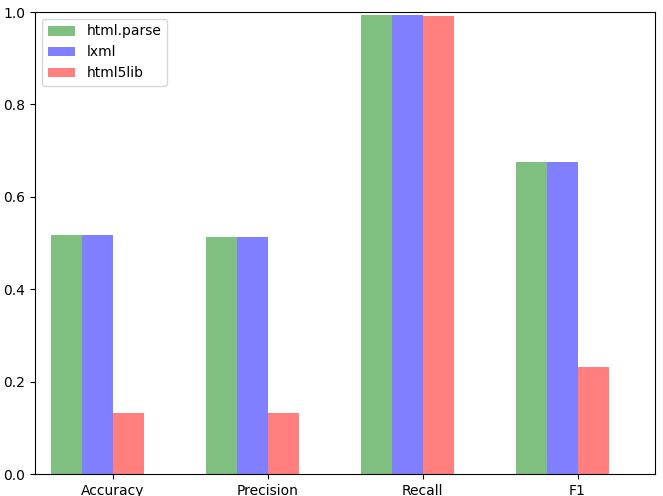
\includegraphics[width=4.6in]{resultados-beautifulsoup.jpg}
    \caption{Gráfica - Resultados de la evaluación de Beautiful Soup}
    \label{img:grafica - resultados de la evaluacion de beautiful soup}
\end{figure}

Por otro lado, respecto a las métricas dependientes del entorno, el uso de memoria RAM, al igual que el uso
de CPU, es similar en todos los analizadores. Véase \ref{img:grafica - resultados de la evaluacion de beautiful soup 2}.

\begin{figure}[tphb]
    \centering
    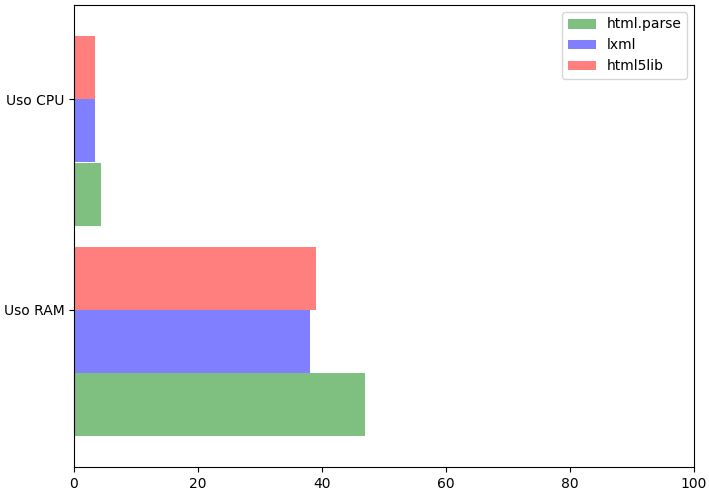
\includegraphics[width=4.6in]{resultados-beautifulsoup2.jpg}
    \caption{Gráfica - Resultados de la evaluación de Beautiful Soup 2}
    \label{img:grafica - resultados de la evaluacion de beautiful soup 2}
\end{figure}

\section*{jusText}

El siguiente paquete sometido a análisis será \textbf{jusText}, el cual debemos instalar e importar en el
fragmento de código respectivo. En cuanto a su instalación, es muy sencilla, simplemente se debe ejecutar
la siguiente instrucción en la línea de comandos: \emph{\$ pip install justext}.

Como se observa en el fragmento de código \ref{cod:funcion de ejecucion de jusText}, la forma en la que
se extrae texto de documentos HTML es muy similar a las vistas anteriormente. La principal diferencia es
que en este caso \textbf{jusText}, previamente a la extracción, realiza las siguientes acciones:

\begin{itemize}
    \item Clasificación de bloques.
    \item Preprocesamiento de bloques de cabecera.
    \item Reclasificación de bloques.
    \item Postprocesamiento de bloques de cabecera.
\end{itemize}

\begin{codefloat}
    \inputencoding{latin1}
    \lstinputlisting[style=CppExample, showstringspaces=false]{scripts/script-justext.py}
    \inputencoding{utf8}
    \caption{Función de ejecución de jusText}
    \label{cod:funcion de ejecucion de jusText}
\end{codefloat}

Como el resto de algoritmos, para conservar la información obtenida y no ejecutar el código múltiples 
veces, el diccionario obtenido se almacena en un archivo \emph{json} propio del paquete. De esta forma, 
el \emph{justext.json} conserva todos los fragmentos de texto obtenidos del minado web anterior.

Una vez ejecutado el algoritmo, se realizan todos los cálculos pertinentes y se determinan las puntuaciones 
obtenidas. En el caso de \textbf{jusText}, los resultados obtenidos se muestran en la tabla 
\ref{tab:tabla - resultados de la evaluacion de justext}.

\begin{table}[h]
    \begin{center}
      \begin{tabular}{| c | c | c | c | c | c | c | c |} \hline 
       \textbf{Nombre} & \textbf{Accuracy} & \textbf{Precision}  & \textbf{Recall} & \textbf{F1} & \textbf{RAM(\%)} & \textbf{CPU(\%)} & \textbf{Time Exec.(s)} \\ \hline
       jusText & 0.7668 & 0.8649 & 0.8573 & 0.8610 & 45.1 & 0.5 & 2.9546 \\ \hline
      \end{tabular}
      \caption{Tabla - Resultados de la evaluación de jusText}
      \label{tab:tabla - resultados de la evaluacion de justext}
    \end{center}
\end{table}

En forma de gráfica, se muestra en la figura \ref{img:grafica - resultados de la evaluacion de justext}
los cálculos obtenidos en referencia a las métricas independientes del entorno de ejecución. Con un simple
vistazo, es posible determinar que el algoritmo de \textbf{jusText} realiza un buen trabajo en al selección
de contenido relevante. 

\begin{figure}[tphb]
    \centering
    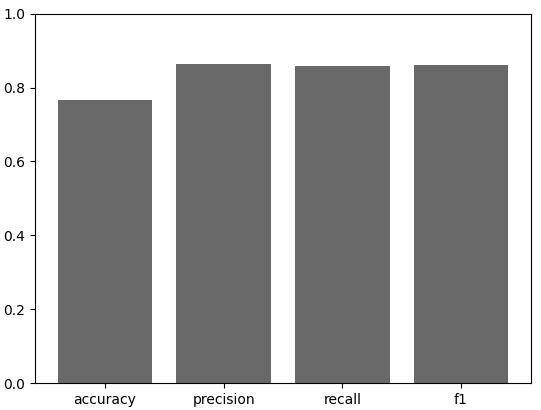
\includegraphics[width=5in]{resultados-justext.jpg}
    \caption{Gráfica - Resultados de la evaluación de jusText}
    \label{img:grafica - resultados de la evaluacion de justext}
\end{figure}

Por otro lado, con respecto a las métricas dependientes del entorno de ejecución, se debe remarcar que
\textbf{jusText} es un paquete de minado web muy bien optimizado. A pesar de realizar todo el trabajo previo
a la extracción, mantiene un buen tiempo de ejecución y escaso uso de la CPU.

\section*{html\_text}

El siguiente paquete sometido a análisis será \textbf{html\_text}, el cual debemos instalar e importar en 
el fragmento de código respectivo. En cuanto a su instalación, simplemente se debe ejecutar la siguiente 
instrucción en la línea de comandos: \emph{\$ pip install html-text}.

\begin{codefloat}
    \inputencoding{latin1}
    \lstinputlisting[style=CppExample, showstringspaces=false]{scripts/script-htmltext.py}
    \inputencoding{utf8}
    \caption{Función de ejecución de html\_text}
    \label{cod:funcion de ejecucion de htmltext}
\end{codefloat}

En el fragmento de código \ref{cod:funcion de ejecucion de htmltext} se muestra como \textbf{html\_text} 
extrae texto de los diferentes documentos HTML. La función \emph{extract\_text()} emplea expresiones 
\emph{xPath} y normalizaciones de espacio para obtener una mejor calidad en los resultados.

Una vez ejecutado el algoritmo, se realizan todos los cálculos pertinentes y se determinan las puntuaciones 
obtenidas. En el caso de \textbf{html\_text}, los resultados obtenidos se muestran en la tabla 
\ref{tab:tabla - resultados de la evaluacion de htmltext}.

\begin{table}[h]
    \begin{center}
      \begin{tabular}{| c | c | c | c | c | c | c | c |} \hline 
       \textbf{Nombre} & \textbf{Accuracy} & \textbf{Precision}  & \textbf{Recall} & \textbf{F1} & \textbf{RAM(\%)} & \textbf{CPU(\%)} & \textbf{Time Exec.(s)} \\ \hline
       html\_text & 0.5166 & 0.513 & 0.9928 & 0.6765 & 44.9 & 0.5 & 1.1800 \\ \hline
      \end{tabular}
      \caption{Tabla - Resultados de la evaluación de html\_text}
      \label{tab:tabla - resultados de la evaluacion de htmltext}
    \end{center}
\end{table}

Tanto en la tabla \ref{tab:tabla - resultados de la evaluacion de htmltext} como en su correspondiente
gráfica \ref{img:grafica - resultados de la evaluacion de htmltext}, podemos observar que el algoritmo
cumple asequiblemente con unos requisitos mínimos con respecto a aquellas métricas no dependientes del
entorno de ejecución.

\begin{figure}[tphb]
    \centering
    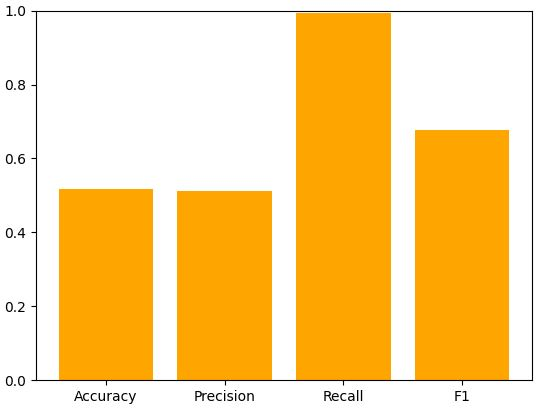
\includegraphics[width=5in]{resultados-htmltext.jpg}
    \caption{Gráfica - Resultados de la evaluación de html\_text}
    \label{img:grafica - resultados de la evaluacion de htmltext}
\end{figure}

En cuanto a las métricas dependientes de entorno, es cierto que el algoritmo emplea pocos recursos, y su
tiempo de ejecución es reducido. Esto se debe a que su heurística es simple, el uso único de expresiones
\emph{xPath} optimiza los recursos. ¿Compensa sobre la calidad de la extracción? Lo veremos en al siguiente
sección, cuando comparemos la \emph{performance} de todos los paquetes.

\section*{html2text}

El siguiente paquete sometido a análisis será \textbf{html2text}, el cual debemos instalar e importar en 
el fragmento de código respectivo. En cuanto a su instalación, simplemente se debe ejecutar la siguiente 
instrucción en la línea de comandos: \emph{\$ pip install html2text}.

\begin{codefloat}
    \inputencoding{latin1}
    \lstinputlisting[style=CppExample, showstringspaces=false]{scripts/script-html2text.py}
    \inputencoding{utf8}
    \caption{Función de ejecución de html2text}
    \label{cod:funcion de ejecucion de html2text}
\end{codefloat}

En el fragmento de código \ref{cod:funcion de ejecucion de html2text} se muestra como \textbf{html2text}
extrae texto de los diferentes documentos HTML. Si recordamos, \textbf{html2text} no se caracteriza por
disponer de una heurística compleja, el algoritmo simplemente hace uso de \emph{html.parse} para analizar
el documento y envolver todos los párrafos del texto proporcionado.

\begin{table}[h]
    \begin{center}
      \begin{tabular}{| c | c | c | c | c | c | c | c |} \hline 
       \textbf{Nombre} & \textbf{Accuracy} & \textbf{Precision}  & \textbf{Recall} & \textbf{F1} & \textbf{RAM(\%)} & \textbf{CPU(\%)} & \textbf{Time Exec.(s)} \\ \hline
       html2text & 0.5105 & 0.5107 & 0.9804 & 0.6715 & 44.6 & 1.8 & 4.4020 \\ \hline
      \end{tabular}
      \caption{Tabla - Resultados de la evaluación de html2text}
      \label{tab:tabla - resultados de la evaluacion de html2text}
    \end{center}
\end{table}

Los resultados mostrados, tanto en la tabla \ref{tab:tabla - resultados de la evaluacion de html2text} como
en la gráfica \ref{img:grafica - resultados de la evaluacion de html2text}, hacen reflejo de la simplicidad
de su heurística. A pesar de todo ello, la calidad en general de la extracción no está muy lejos de la media.

\begin{figure}[tphb]
    \centering
    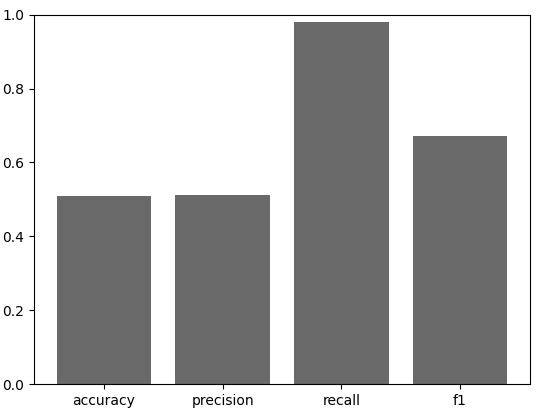
\includegraphics[width=4.7in]{resultados-html2text.jpg}
    \caption{Gráfica - Resultados de la evaluación de html2text}
    \label{img:grafica - resultados de la evaluacion de html2text}
\end{figure}

\section*{Readability}




